% Por enquanto esse capítulo está separado

\chapter{Biblioteca digital do Participa.br}
\label{cap:bibparticipabr}

Nesse capítulo será apresentado alguns resultados dos levantamentos iniciais sobre os mecanismos formais de participação, além de apresentar um primeiro protótipo sobre a biblioteca digital do Participa.br. Para esse primeiro protótipo, os metadados considerados serão apresentados na seção \ref{sub:metadadospbr}. Mais adiante uma proposta para interoperabilidade do Participa.br (Noosfero) e a biblioteca digital através de um plugin que implementa o protocolo OAI-PMH é visto na seção \ref{sec:interparticipa}. Já o primeiro protótipo da biblioteca digital de participação social é visto na seção \ref{sub:prototipo_biblioteca}.

Também constam recomendações e sugestões sobre preservação de artefatos digitais visando uma sobrevida maior, e beneficiando não somente documentos textuais, mas todo e qualquer tipo de informação multimídia (áudio, vídeo, imagem, etc.).

\section{Mecanismos formais de participação}

Compilar todo o conteúdo do capítulo 1 e 2 do TCC 1 nessa área.

\section{Arquitetura da Informação sobre Participação Social}

Atualmente não existe um lugar centralizado para os usuários buscarem informações sobre os mecanismos formais de participação. Cada órgão possui seu próprio repositório de informações, disponibilizados em diversas formatos digitais, sendo elas: planilhas, documentos, páginas HTML, entre outros. Muito desses órgãos disponibilizam informações desatualizadas e incompletas, outros já disponibilizam os dados de formas estruturadas e completas como no caso do Conselho Nacional de Saúde. 

Aliado ao crescente número de mecanismos formais de participação durante a última década, ficou evidente que encontrar informações sobre esses mecanismos se torna dispendioso. Por isso é necessário criar um canal onde os usuários possam acessar todos os dados de maneira centralizada, e que as informações sobre os mecanismos formais possam estar sempre atualizadas, tudo isso dentro do Participa.br.

Para criação desse canal centralizado para disponibilização dos mecanismos formais de participação foi feito um primeiro levantamento. Esse levantamento levou em consideração as informações disponibilizadas nos diversos portais dos canais de participação (mais especificamente sobre conselhos, conferências e ouvidorias) e nas entrevistas que foram realizadas durante o período de confecção da primeira versão desta monografia.

Após esse levantamento inicial, foi notado que os sites são muito heterogêneos e que a estrutura assumida por cada canal é peculiar àquele site. De um modo geral, as informações de participação social incorporam páginas web e arquivos textos com a maior parte das informações. Além dessa forma, muitos sites contém arquivos multimídia contendo áudio, vídeo e imagens como documentários sobre as reuniões dos conselhos, palestras, entre outros, que podem ser colocados para visualização dos usuários.

É importante ressaltar que, num primeiro momento, para apresentação do protótipo, foram considerados apenas alguns objetos digitais construídos especialmente para essa biblioteca digital cujos conteúdos são exatamente as informações essenciais do canal de informação, tais como o URL, os dados do gestor e outras informações relevantes. Portanto, esse foi o nível de granularidade definido para o objeto digital nesse primeiro protótipo de biblioteca digital.

\section{Metadados de Participação Social}
\label{sub:metadadospbr}

A fim de atender ao propósito dessa pesquisa, foi feito um levantamento nos principais mecanismos formais de participação, a fim de identificar quais seriam os metadados relevantes a serem incluídos na biblioteca digital do Participa.br. Além desse levantamento em sites, alguns gestores foram consultados para que opinassem sobre que tipo de informações eles gostariam de ver respondidas com a biblioteca digital. O resultado desse levantamento permitiu elencar os metadados que estão apresentados nas Tabelas \ref{tab:metadata_dc_mecanismo} a \ref{tab:metadata_pbr_ouvidorias} para conselhos, conferências e ouvidorias, considerados os principais canais de participação para efeito de teste da biblioteca digital que está sendo proposta.

Em função das características citadas, para o catalogação dos dados do Participa.br sugere-se a utilização dos formatos de banda 2, mais especificamente o Dublin Core, que deve ser tomado como referência para criação de qualificadores para os conteúdos de participação social.

Na tabela \ref{tab:metadata_dc_mecanismo} serão apresentados os metadados significativos para conselhos, conferências e ouvidorias que tem uma correlação com metadados do padrão Dublin Core.

\newcolumntype{'}{!{\vrule width 2pt}}
\makeatother 

\begin{table}[H]
	\begin{center}
	\caption[Metadados Participa com relação DC para os mecanismos formais]{Metadados Participa com Relação DC para conselhos, conferências e ouvidorias}
    \begin{tabular}{'l|p{9cm}'}\thickhline
    \rowcolor[HTML]{BFBFBF}
    \multicolumn{1}{!{\vrule width 2pt}c!{\vrule width 1pt}}{\textbf{METADADO}} & 
  \multicolumn{1}{!{\vrule width 0pt}c!{\vrule width 2pt}}{\textbf{DESCRIÇÃO}} \\ \noalign{\hrule height 3pt}
    dc.title & Nome do mecanismo formal de participação \\ \hline
    dc.creator & Órgão o qual aquele canal formal faz parte. \\ \hline
    dc.subject & Palavras chaves que relacionam ao canal formal. \\ \hline
    dc.description & Uma pequena descrição, finalidade ou objeto o qual aquele mecanismo formal está ligado.\\ \hline
    dc.date & Data de criação do canal de participação. \\ \hline
    dc.type & Tipo de caráter que o canal de participação possui (representativa, consultiva, deliberativa, participativa, etc.). \\ \hline
    dc.identifier & URL/URI do canal de participação. Sítio Eletrônico onde se encontra a página do canal formal de participação. \\ \hline
    dc.language & Linguagem utilizada descrição do canal formal de participação (previsão para outras linguagens no futura.) \\ \hline
    dc.relation & Define ligação entre canais formais. \\ \hline
    dc.rights & Tipo de licença para divulgação do conteúdo daquele canal. \\ \noalign{\hrule height 2pt}
    \end{tabular}
    \end{center}
    \label{tab:metadata_dc_mecanismo}
\end{table}

Como o padrão Dublin Core não foi suficiente para mapear todas as referências necessárias para os artefatos digitais, foi definida uma tabela específica para cada um dos três tipos de mecanismos formais de participação, usando um conjunto de metadados específico, identificados com o prefixo pbr como uma alusão ao projeto Participa.br. Esses metadados específicos possuem a desvantagem de não serem interoperáveis fora do contexto dos canais de participação social que estiverem conectados à rede de bibliotecas digitais planejada para o Participa (essa discussão será feita mais adiante na seção \ref{cap:extbibparticipa}), no entanto, eles descrevem melhor as demais referências que não foram mapeadas no Dublin Core.

Na tabela \ref{tab:metadata_pbr_conselho} estão os metadados do Participa.br, que não possuem relação com o Dublin Core para conselhos.

\begin{table}[H]
\begin{center}
    \caption{Metadados Participa.br para conselhos}
    \begin{tabular}{'l|p{9cm}'}\thickhline
    \rowcolor[HTML]{BFBFBF}
    \multicolumn{1}{!{\vrule width 2pt}c!{\vrule width 1pt}}{\textbf{METADADO}} & 
  \multicolumn{1}{!{\vrule width 0pt}c!{\vrule width 2pt}}{\textbf{DESCRIÇÃO}} \\ \noalign{\hrule height 3pt}
    pbr.sigla & Sigla do mecanismo formal de participação \\ \hline
    pbr.competencia & Competências e atribuições a qual o conselho responde, geralmente regidas em lei. \\ \hline
    pbr.composicao & Composição entre os membros de um conselho, também geralmente são regidas em lei (Por exemplo: membros da sociedade civil, membros da esfera pública). \\ \hline
    pbr.escolha & Forma de escolha dos membros (Por exemplo: votação, indicação, etc.). \\ \hline
    pbr.mandato & Nome das pessoas que estão fazendo parte do conselho em um determinado tempo. \\ \hline
    pbr.legislacao & Todas as leis (leis, decretos, portarias, etc.) que estão relacionados aquele conselho. \\ \hline
    pbr.endereco & Esse metadado possui informações sobre o endereço físico a qual aquele conselho está instalado (bairro, cidade, CEP, rua, etc.) e também inclui informações sobre telefone e e-mail do conselho. \\ \hline
    pbr.dtreuniao & Data de reuniões, audiências, etc. \\ \noalign{\hrule height 2pt}
    \end{tabular}
    \label{tab:metadata_pbr_conselho}
\end{center}
\end{table}

%Tabela 3.2 - Metadados Participa para conselhos

Na tabela \ref{tab:metadata_pbr_conferencias} estão apresentados os metadados Participa.br para conferências e que não tem uma correlação com metadados do padrão Dublin Core.

\begin{table}[H]
\begin{center}
    \caption{Metadados Participa.br para conferências}
    \begin{tabular}{'l|p{9cm}'}\thickhline
    \rowcolor[HTML]{BFBFBF}
    \multicolumn{1}{!{\vrule width 2pt}c!{\vrule width 1pt}}{\textbf{METADADO}} & 
  \multicolumn{1}{!{\vrule width 0pt}c!{\vrule width 2pt}}{\textbf{DESCRIÇÃO}} \\ \noalign{\hrule height 3pt}
    pbr.sigla & Sigla do mecanismo formal de participação \\ \hline
    pbr.competencia & Competências e atribuições a qual o conferência responde, geralmente regidas em lei. \\ \hline
    pbr.tema & Tema central daquela conferência. \\ \hline
    pbr.composicao & É composto pelos membros que fizeram parte da edição daquela conferência. \\ \hline
    pbr.legislacao & Todas as leis (Leis, decretos, portarias, etc.) que estão relacionados aquela conferência. \\ \hline
    pbr.endereco & Esse metadado possui informações sobre o endereço físico a qual aquele conselho está instalado (bairro, cidade, CEP, rua, etc.) incluso informações sobre telefone e e-mail do conselho. \\ \hline
    pbr.dtreuniao & Possui a data de reuniões, audiências, etc. \\ \noalign{\hrule height 2pt}
    \end{tabular}
    \label{tab:metadata_pbr_conferencias}
\end{center}
\end{table}

% Tabela 3.3 - Metadados sobre conferências

Na tabela \ref{tab:metadata_pbr_ouvidorias} contém metadados Participa.br para catalogação de informações sobre ouvidorias. Assim como nas conselhos e conferências, alguns significados são compatíveis.

\begin{table}[H]
\begin{center}    
    \caption{Metadados Participa.br para ouvidorias}
    \begin{tabular}{'l|p{9cm}'}\thickhline
    \rowcolor[HTML]{BFBFBF}
    \multicolumn{1}{!{\vrule width 2pt}c!{\vrule width 1pt}}{\textbf{METADADO}} & 
  \multicolumn{1}{!{\vrule width 0pt}c!{\vrule width 2pt}}{\textbf{DESCRIÇÃO}} \\ \noalign{\hrule height 3pt}
    pbr.sigla & Sigla do mecanismo formal de participação \\ \hline
    pbr.competencia & Competências e atribuições a qual a ouvidoria responde, geralmente regidas em lei. \\ \hline
    pbr.responsaveis & Nome das pessoas responsáveis pela ouvidoria. \\ \hline
    pbr.legislacao & Todas as leis (leis, decretos, portarias, etc.) que estão relacionados com aquela ouvidoria. \\ \hline
    pbr.endereco & Informações sobre o endereço físico a qual aquele conselho está instalado (bairro, cidade, CEP, rua, etc.) incluso outras informações, como telefone e e-mail do conselho. \\ \noalign{\hrule height 2pt}
    \end{tabular}
    \label{tab:metadata_pbr_ouvidorias}
\end{center}
\end{table}

% Tabela 3.4 - Metadados Participa para ouvidorias

Em versões futuras dessa biblioteca digital serão tratados objetos multimídia tais como filmes e fotos para que esses também possam ser localizados na biblioteca digital. Além disso, pretende-se criar um thesaurus, e um vocabulário controlado para melhorar o proecesso de busca indexada. Do ponto de vista das consultas, foram pensadas inicialmente a apresentação dos canais formais com base nos seguintes alternativas de chegada às informações dos canais formais:

\begin{itemize}
	\item Relação de canais formais por tipo (conferência, conselho, ouvidoria, etc). 
	\item Relação de canais formais por ordem alfabética (independente do tipo de canal formal).
	\item Relação de canais formais por ordem cronológica de criação.
	\item Relação de canais formais pela origem (por ministério, por exemplo).
	\item Relação de canais formais por região/estado
	\item Relação de canais formais por assunto (mais social, mais ligado a questões políticas, etc.).
\end{itemize}

Os dados dos canais formais serão apresentados em níveis para facilitar o acesso às informações. No primeiro nível sugere-se a apresentação dos metadados essenciais, como o índice geral, o link para tela principal do canal de participação e outras informações essenciais como o nome e a eventual sigla do canal. No segundo nível será aberto um detalhamento maior contendo as informações essenciais que foram recuperadas das páginas de rosto de cada canal. Nesse caso, aparecem informações sobre a legislação essencial, sobre os coordenadores e seus dados de acesso (telefone, endereço, etc). Será dada ainda a opção de apresentação de um terceiro nível, onde for necessário, com a informação completa do site recuperada e inserida dentro da biblioteca digital. Dessa forma, o usuário pode realizar consultas de formas variadas e poderá inclusive chegar na página web do canal sem precisar passar pelos passos anteriores.

\section{Interoperabilidade entre o Participa.br e mecanismos de participação social}
\label{sec:interparticipa}

Como prova de conceito, num primeiro momento foi elaborado um protótipo de biblioteca digital na versão centralizada com uso de software livre, mais especificamente de algum dos softwares levantados e listados no Anexo \ref{Att:anexobibliotecas} deste trabalho (maiores detalhes sobre essa construção estão descritas na seção \ref{sub:prototipo_biblioteca}). No entanto, em função da dinâmica de modificação das informações de participação social, é importante assumir a estratégia de se criar um modelo de interação entre os canais de participação social e o portal Participa.br, considerando os primeiros como provedores de dados e o portal como um provedor de serviços, como está representado na figura \ref{fig:modeloaipmh}.

\graphicspath{{figuras/}}
\begin{figure}[H]
\centering
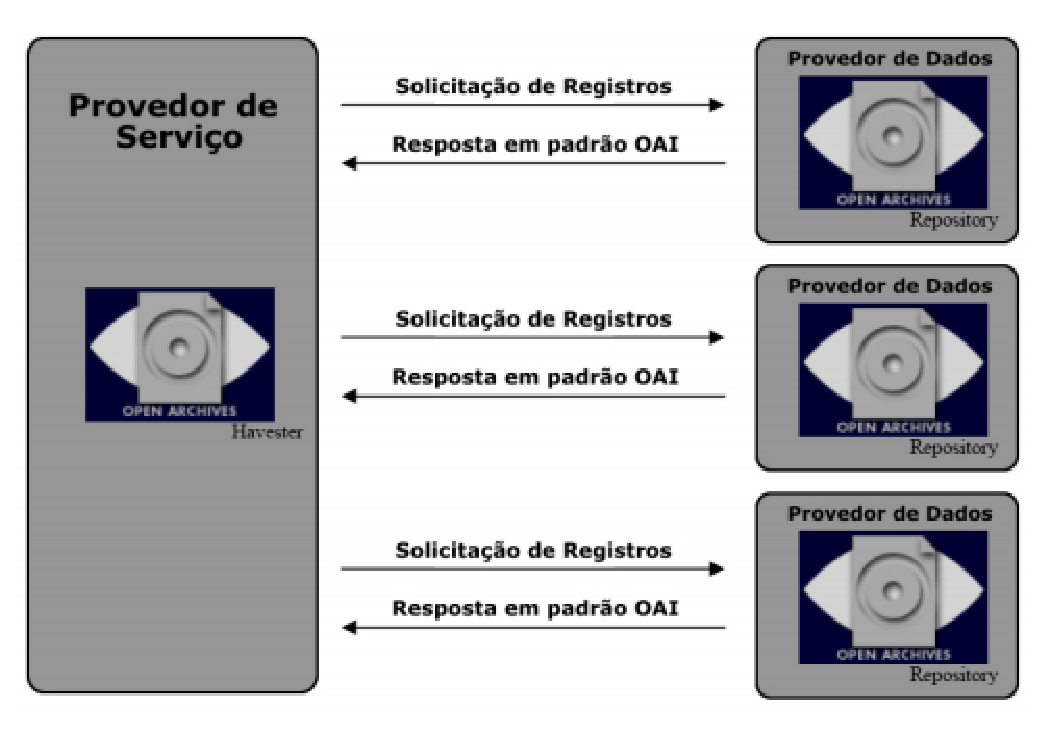
\includegraphics[width=0.9\textwidth]{modelo-oaipmh}
\caption[Modelo de comunicação OAI-PMH entre o portal e os mecanismos]{Modelo de comunicação OAI-PMH entre o portal e os canais de participação. Extraído de \cite{renan2009interoperabilidade}}
\label{fig:modeloaipmh}
\end{figure}

Nessa imagem ilustrada pela figura \ref{fig:modeloaipmh}, os canais de participação conteriam em seus portais, um módulo de biblioteca digital que seria elaborado como produto dessa monografia e distribuído para eles via promoções feitas pelos gestores responsáveis pelo acompanhamento dos canais formais, por exemplo. Com esse módulo acoplado, os canais de participação passam a ter um site pré-configurado e pronto para comportar informações relevantes de uso interno e externo, pelo preenchimento de metadados ou informações tais como telefones de contato, nomes dos conselheiros, reuniões, atas de reuniões e outras informações em formatos variados que possam e necessitem ser catalogadas localmente.

Por outro lado, o portal Participa terá acoplado a si um módulo da biblioteca digital que o tornará um provedor de serviços capaz de interagir com os provedores de dados e coletar metadados essenciais sobre cada um desses provedores de dados, por meio do protocolo de harvesting OAI-PMH. Dessa forma, o Participa poderá auxiliar os canais de participação na organização de seus conteúdos de informação e, ao mesmo tempo, poderá ser um provedor de informações atualizadas sobre os diversos canais de participação, uma vez que as colheitas de dados nos provedores podem ser feitas em qualquer instante desejado. Vale lembrar que o OAI-PMH foi preferido em relação aos outros padrões, como é o caso do Z39.50, porque permite escalabilidade e uma maior liberdade de troca de informações e uma interoperabilidade com baixo grau de envolvimento entre as partes, preservando, dessa forma, a autonomia de cada um dos canais de participação. No caso do OAI-PMH, este padrão foi escolhido já como padrão a ser utilizado para implementação. 

No entanto, para viabilizar essa solução, é importante que, após definida a interface da biblioteca digital, haja uma campanha de distribuição dessas bibliotecas entre os canais de participação interessados, preferencialmente criando-se elementos de motivação que incentivem a adoção máxima desse ambiente de organização de conteúdos e interoperabilidade.

\section{Adaptando a biblioteca digital para um provedor de dados}

\section{Adaptando o Noosfero para um provedor de serviços}

Para viabilizar a construção desse módulo OAI-PMH no Noosfero que utiliza a linguagem Ruby, vista na seção \ref{sec:linguagemruby}, existem alternativas como a gema (\textit{gem}) OAI \footnote{Maiores Informações em: \url{https://github.com/code4lib/ruby-oai}}, que implementam várias funcionalidades entre provedores de dados e serviços pertencentes ao padrão do OAI. No caso do Participa.br, os provedores de dados vão utilizar os protocolos já implementados pelos softwares de bibliotecas digitais e no Noosfero utilizado pelo Participa.br será implementado um plugin, visto na seção \ref{sub:arquiteturaplugin} que irá utilizar a implementação do OAI.

A escolha dessa implementação ser feita em um plugin, deve-se ao fato da necessidade de transformar o Participa.br em uma biblioteca digital seja exclusiva do Participa.br neste primeiro momento. No entanto, nada impede de outras instâncias utilizem esse plugin.

% A princípio separei em 3 capítulos o desenvolvimento do plugin, já
%

\subsection{O plugin de interoperabilidade}

Nesse sub-seção será abordado todo o desenvolvimento do plugin na plataforma noosfero (Conceituar e justificar o seu desenvolvimento).

\subsection{Código do plugin}

Explicação sobre o desenvolvimento do código do plugin

\subsection{Testes do plugin}

Explicação sobre os testes a ser desenvolvidos (unitário, integração, cucumber, entre outros)

\section{Aplicação da arquitetura da biblioteca digital}

Explicação sobre o funcionamento do plugin

